\documentclass{report}
\usepackage{ugentstyle}


\newenvironment{grammarfigure} % Environment that changes the caption name to "Grammatica" for figures
{
	\renewcommand{\figurename}{Grammatica}
	\begin{figure}[h]
}
{
	\end{figure}
	\renewcommand{\figurename}{Figuur}
}


% commando om vraag-antwoord situaties te behandelen
\newcommand{\QA}[2]{
	\noindent\fbox{
		\parbox{\linewidth}{
			\textbf{Q:} #1
			
			 \textbf{A:} #2
		}
	}
}

\begin{document}
	\maketitle{Compilers}
	\tableofcontents
	\part{Theorie}
	\chapter{Inleiding}
\section{Compilers}
Voorbeelden van functies die een statische compiler moet bevatten:
	\begin{itemize}
		\item Broncode omzetten in uitvoerbare fouten:
		\begin{itemize}
			\item met dezelfde semantiek
			\item zo snel mogelijk
			\item en/of zo compact, debugbaar, portable, veilig, ... mogelijk
			\item en linkbaar.
		\end{itemize}
		\item Syntaxfouten moeten herkent worden.
	\end{itemize}

\section{Basiswerking compilers}
\begin{figure}[h]
	\centering
	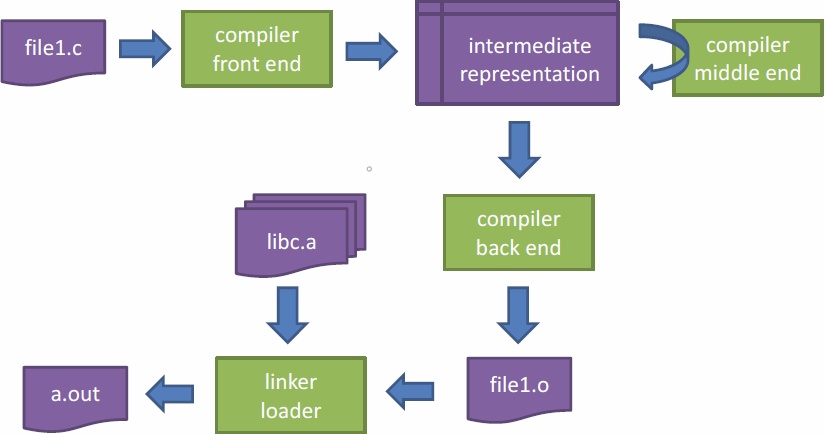
\includegraphics[width=0.5\textwidth]{basiswerking_compilers}
	\caption{De basiswerking van een compiler.} 
	\label{fig:basiswerking_compilers}
\end{figure}
Op figuur \ref{fig:basiswerking_compilers} is de vereenvoudigde basiswerking van een compiler te zien. Een \textbf{C} bestand wordt eerst door de \uline{compiler front end} gestuurd, die het bestand zal omvormen tot een intermediaire representatie. Deze representatie wordt dan door de \uline{compiler back end} gestuurd om zo assembly of objectcode te genereren. De \uline{linker loader} zal deze objectcode samenvoegen met eventuele andere libraries om zo een uitvoerbaar programma te hebben. 

\QA{Waarom wordt de front end en back end opgesplitst?}
{Op die manier is de compiler modulair: Enerzijds moet bij een andere programmeertaal enkel de front end aangepast worden en anderzijds moet bij het wijzigen van de architectuur (de onderliggende processor) enkel de back end aangepast worden.}


\section{Abstract Syntax Tree}
De eerste stap van elke compiler is het omvormen van de broncode naar een \textbf{Abstract Syntax Tree (AST)}. Veronderstel volgende code, en de daarbijhorende AST die te zien zijn op figuur \ref{fig:abstract_syntax_tree}. Elke knoop van een AST stelt een bepaalde geldige operatie voor, die afhankelijk is van de gekozen programmeertaal.
\begin{figure}[h]
	\centering
	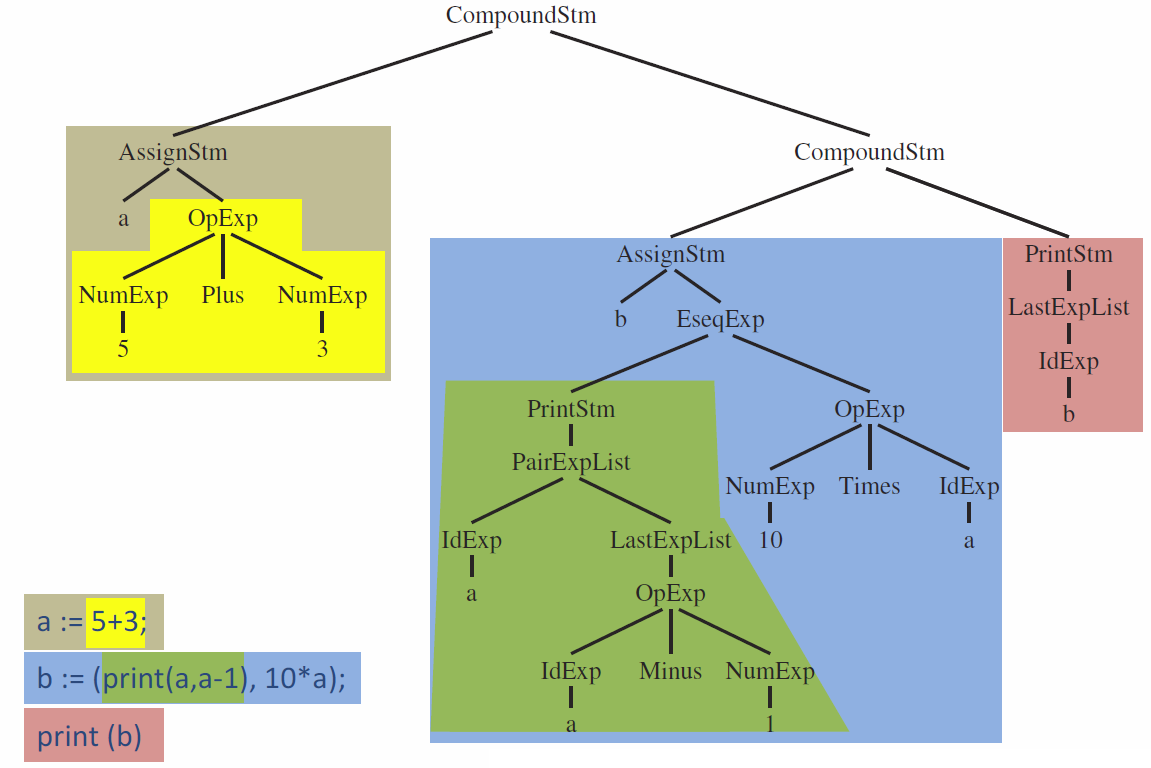
\includegraphics[width=0.8\textwidth]{abstract_syntax_tree}
	\caption{De boomvoorstelling van een eenvoudig, lusloos programma. De gekleurde deelbomen komen overeen met de gekleurde segmenten in de code zelf. Als toekenningsoperator wordt er gekozen voor $:=$ dat vanaf nu als één geheel moet beschouwd worden.}
	\label{fig:abstract_syntax_tree}
\end{figure}

\subsection{Contextvrije grammatica's}
Om een AST op te stellen moet de notie van \textbf{tokens} ingevoerd worden. Een token is eenvoudig gezien een bepaald symbool dat een betekenis heeft. De tokens van de code uit figuur \ref{fig:abstract_syntax_tree} zijn te zien in tabel \ref{table:tokens}
\begin{table}[h]
	\centering
	\begin{tabular}{l | l | l}
		symbolen(ascii) & token & waarde \\
		\hline
		a & id & string a \\
		:= & := & \\
		5 & num & integer 5 \\
		+ & + & \\
		3 & num & integer 3 \\
		; & ; & \\
		b & id & string b \\
		( & ( & \\
		print & print & \\
		- & - & \\
		* & * & \\
		  & whitespace & \\
	\end{tabular}
	\caption{De tokens die voorkomen uit het programma van figuur \ref{fig:abstract_syntax_tree}}
	\label{table:tokens}
\end{table}
Uit de theorie van de generatieve grammatica's weten we dat er zowel terminale als niet-terminale tokens bestaan:
\begin{itemize}
	\item \textbf{Terminale tokens} zijn symbolen die een blad voorstellen in de AST. Deze tokens hebben als eigenschap dat ze geen verdere tokens kunnen genereren en vormen dan ook het alfabet van het programma.
	\item \textbf{Niet-terminale tokens}, kortweg niet-terminalen genoemd, zijn de regels die de taal definiëren en zijn de niet-bladeren van de AST. Niet-terminalen hebben als eigenschap dat ze letters van het alfabet kunnen genereren.
\end{itemize}
Op figuur \ref{fig:contextvrije_grammatica} zijn een aantal terminalen en niet-terminalen te zien. De niet-terminale token \textit{CompoundStm} bestaat bijvoorbeeld uit twee \textit{Stm} tokens, gescheiden door een punt komma. Deze twee \textit{Stm} tokens kunnen in deze vereenvoudigde programmeertaal enkel een \textit{AssignStm} of \textit{PrintStm} zijn. Bij \textit{AssignStm} wordt er een terminale token verwacht in de vorm van een variabele identifier, gevolgd door de toekenningsoperator en een \textit{Exp} token. Enkel deze \textit{Exp} kan nog vier vormen aanneemen: \textit{IdExp}, \textit{NumExp}, enz...
{
\begin{figure}[h]
	\definecolor{cvred}{RGB}{215,149,146}
	\definecolor{cvblue}{RGB}{145,202,219}
	\centering
	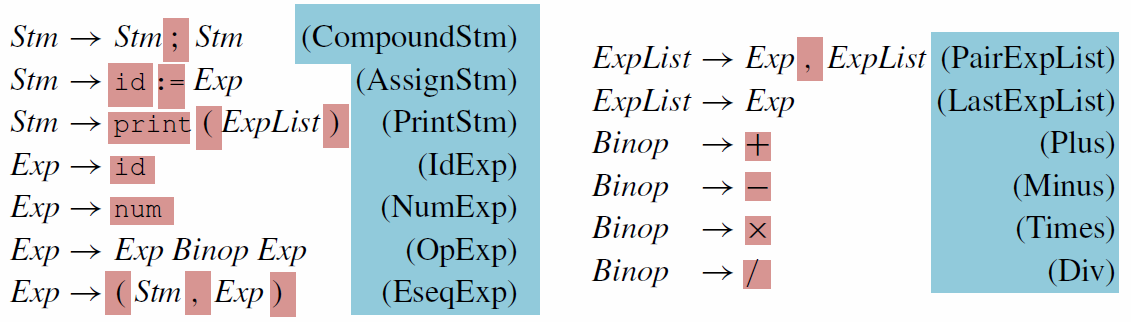
\includegraphics[width=0.8\textwidth]{contextvrije_grammatica}
	\caption{De rood omkaderde symbolen zijn {\color{cvred} terminalen} terwijl de blauw omkaderde {\color{cvblue}niet-terminalen} zijn.} 
	\label{fig:contextvrije_grammatica}
\end{figure}
}
Dit wordt uitgewerkt voor de eerste toekenningsoperatie uit figuur \ref{fig:abstract_syntax_tree} en is te zien op figuur \ref{fig:contextvrije_grammatica_voorbeeld}.
\begin{figure}[h]
	\centering
	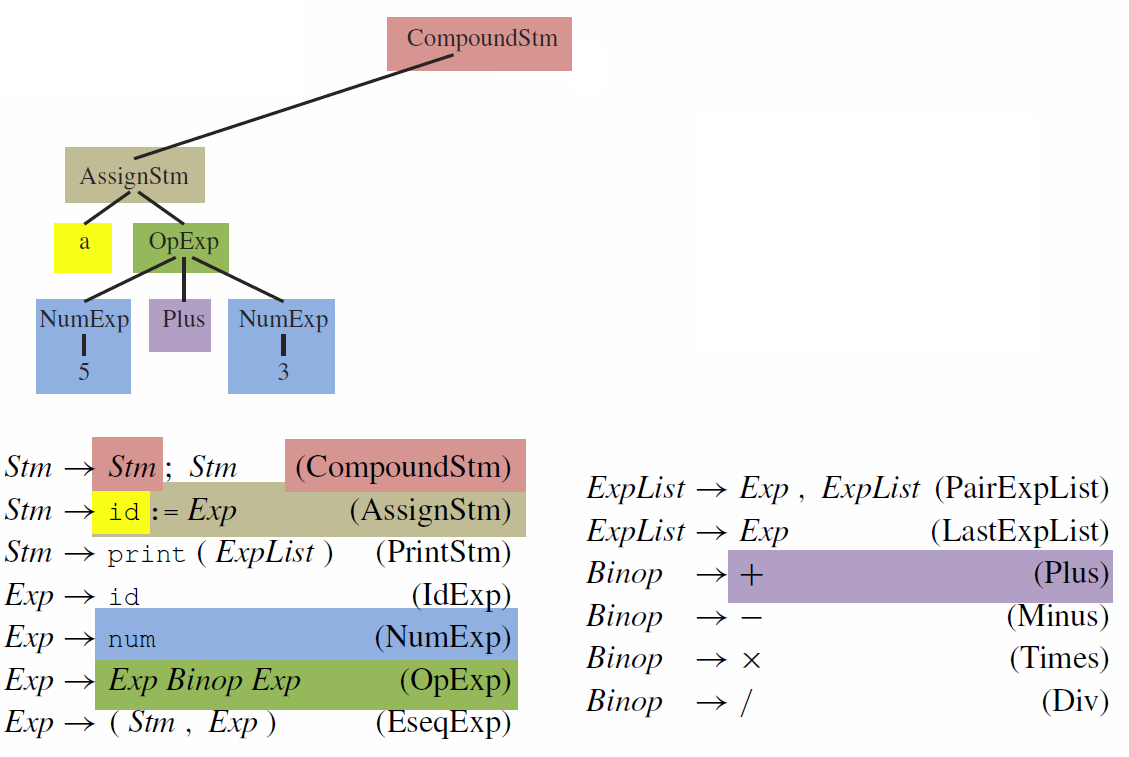
\includegraphics[width=0.8\textwidth]{contextvrije_grammatica_voorbeeld}
	\caption{Illustratie van contextvrije grammatica op de eerste toekenningsoperatie uit figuur \ref{fig:abstract_syntax_tree}.} 
	\label{fig:contextvrije_grammatica_voorbeeld}
\end{figure}

\subsection{Opbouw AST}
Een AST kan nu \textbf{bottom-up} opgemaakt worden door volgende procedure uit te voeren:
\begin{enumerate}
	\item Voor elke mogelijke knoop moet er een struct gemaakt worden zoals bijvoorbeeld:
	
	$$\texttt{A\_stm\_} \qquad \texttt{A\_exp\_} \qquad \texttt{A\_expList\_}$$
	
	\item Elke struct moet bestaan uit
	\begin{itemize}
		\item een enum voor het precieze token te bepalen,
		\item een union voor de verschillende combinaties van tokens in het rechter lid en,
		\item pointers naar kindknopen.
	\end{itemize}
	Dit wordt geïllustreerd in code \ref{lst:vb_struct_AST}.
	\begin{lstlisting}[caption={Voorbeeld van een struct voor een AST.},label={lst:vb_struct_AST}, captionpos=b]
typedef char * string;
typedef struct A_stm_ * A_stm;
typedef struct A_exp_ * A_exp;
typedef struct A_expList_ * A_expList;

struct A_stm_ {
	enum {A_compoundStm, A_assignStm, A_printStm} kind;
	union {
		struct {A_stm stm1, stm2;} compound;
		struct {string id; A_exp exp;} assign;
		struct {A_expList exps;} print;
	} u;
};
	\end{lstlisting}
	\item In de constructor worden de knopen aangemaakt, zoals te zien in code \ref{lst:vb_constructor_AST}.
	\begin{lstlisting}[caption={Voorbeeld van een constructor voor een AST.},label={lst:vb_constructor_AST}, captionpos=b]
A_stm A_CompoundStm(A_stm stm1, A_stm stm2){
	A_stm s = malloc(sizeof(*s));
	s->kind = A_compoundStm;
	s->u.compound.stm1 = stm1;
	s->u.compound.stm2 = stm2;
	return s;
}
	\end{lstlisting}
	
Op deze manier zou de boom uit figuur \ref{fig:abstract_syntax_tree} hardgecodeerd kunnen worden, wat natuurlijk geen goede manier is. Het is de taak van een \uline{lexer} en \uline{parser} om de constructie van een AST te automatiseren, die respectievelijk in hoofdstuk \ref{ch:lexicale_analyse} en \ref{ch:parsing} behandelt worden.

\subsection{Interpreter}
Uit een AST kan een eenvoudige interpreter geschreven worden. Dit stuk is informatief, en wordt niet gevraagd op het examen.
\begin{itemize}
	\item Door de boom postorder diepte-eerst te overlopen, wordt de boom in de juiste manier behandelt.
	\item Het bijhouden van de waarden van variabelen kan via een gelinkte lijst:
	\begin{lstlisting}
typedef struct table * Table_;
struct table {string id; int value; Table_ tail;};
Table_ Table(string id; int value; Table_ tail) {
	Table_ t = malloc(sizeof(*t));
	t->id = id;
	t->value = value;
	t->tail = tail;
	return t;
}
	\end{lstlisting}
	\item Stel nu dat dit de eerste drie regels van een programma zijn:
	\begin{lstlisting}
a := 2;
b := 3;
a := 3;
	\end{lstlisting}
	\item Voor de eerste toekenning bevat de gelinkte lijst slechts één knoop met als sleutel \textit{a} en waarde \textit{2}. 
	\item Bij de tweede toekenning wordt de originele gelinkte lijst meegegeven via de variabele \textit{tail}. Na deze constructor zal de gelinkte lijst twee knopen bevatten.
	\item Na deze constructor bevat de gelinkte lijst drie knopen. Merk op dat er twee knopen zijn met sleutel \textit{a}, maar dat ze elk een verschillende waarde hebben. Aangezien een nieuwe knoop vooraan wordt toegevoegd, zal de interpreter enkel de meest recentste waarde opvragen.
\end{itemize}

\end{enumerate}



	\chapter{Lexicale Analyse}
\section{Lexicale tokens}
\begin{itemize}
	\item Herkennen van een reeks opeenvolgende karakters die een geheel vormen volgens de syntax van een programmeertaal, zoals o.a:
	\begin{itemize}
		\item sleutelwoorden: int, float, for, new, ...
		\item identifiers: foo, n14, variabelenaam
		\item getallen: -37, 0x16L, 10.4, ...
		\item operatoren: +, -, *, \&, \&\&, ...
		\item andere tokens: \{ \} " ; /*  */ / ( ) [ ]
	\end{itemize}

\end{itemize}
	\chapter{Parsing}
\label{ch:parsing}

\section{Inleiding}
Het basisidee van parsing is om een string van tokens te analyseren en kijken of deze syntactisch geldig zijn.

\QA{Waarom gaan we context-vrije grammatica gebruiken in plaats van reguliere expressies om de tokens van een lexer te parsen?}{Reguliere expressies kan geen recurise uitdrukken. Ook kan de eis voor gebalanceerde haakjes niet uitgedrukt worden met reguliere expressies.
}

\section{Context-vrije grammatica}
\begin{itemize}
	\item Een \textbf{taal} is een verzameling \textbf{strings}.
	\item Een \textbf{string} is een eindige sequentie \textbf{symbolen} uit een \textbf{alfabet}.
	\item Analogie met een parser:
	\begin{itemize}
		\item De broncode levert de strings op via lexicale analyse.
		\item De lexicale tokens zijn de symbolen.
		\item Het alfabet is de verzameling tokentypes die gegenereerd worden door de lexicale analyzer.
	\end{itemize}
	\item De taal van een context-vrije
	\item Context-vrije grammatica definieert de \textbf{syntax} van de taal.
\end{itemize}

\subsection{Afleiden van een zin}
Grammatica \ref{fig:vb_grammatica_1} toont een voorbeeldsyntax voor lusloze programma's. Een voorbeeld van een zin is:

\begin{grammarfigure}
	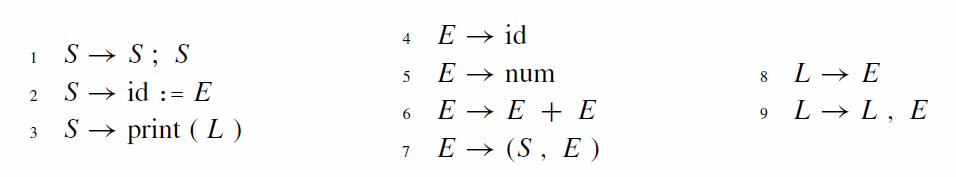
\includegraphics[width=\textwidth]{vb_grammatica_1}
	\caption{Een syntax voor een lusloos programma.}
	\label{fig:vb_grammatica_1}
\end{grammarfigure}


\begin{equation}\label{eqn:voorbeeldzin}
\texttt{id := num ; id := id + (id := num + num, id)}
\end{equation}


die bijvoorbeeld afgeleidt is door de lexer van:
$$\texttt{a := 7; b := c + (d := 5 + 6, d)}$$

Het afleiden van een zin start altijd met een \textbf{startsymbool}, die twee vormen kan aannemen:
\begin{enumerate}
	\item Het startsymbool kan enerzijds het eerste symbool zijn.
	\item Anderzijds wordt het startsymbool expliciet aangeduid zoals bijvoorbeeld $P \rightarrow S\$$, met \$ het stopsymbool.
\end{enumerate}

\begin{lstlisting}[caption={Het afleidingsproces.},label={lst:vb_afleiding},captionpos=b,escapeinside={(*}{*)}]
(*\uline{S}*)
S ; (*\uline{S}*)
(*\uline{S}*) ; id := E
id := (*\uline{E}*) ; id := E
id := num ; id := (*\uline{E}*)
id := num ; id := E + (*\uline{E}*)
id := num ; id := (*\uline{E}*) + (S, E)
id := num ; id := id + ((*\uline{S}*), E)
id := num ; id := id + (id := (*\uline{E}*), E)
id := num ; id := id + (id := E + E, (*\uline{E}*))
id := num ; id := id + (id := (*\uline{E}*) + E, id)
id := num ; id := id + (id := num + (*\uline{E}*), id)
id := num ; id := id + (id := num + num, id)
\end{lstlisting}

Code \ref{lst:vb_afleiding} toont een illustratie van hoe het afleidingsproces te werk gaat, toegepast op voorbeeldzin \ref{eqn:voorbeeldzin}. Bij elke iteratie wordt het niet-terminale token dat onderlijnt is verwerkt.

\QA{Is dit een linkse of een rechtste afleiding?}{Geen van beide, omdat er gekozen kan worden om zowel de meest linkse als de meest rechtse token te verwerken.
}

Figuur \ref{fig:vb_tree_1} toont de bijhorende parse tree. Hier zijn de bladeren ook een verzameling van terminale tokens. De taak van een parser is om de bijhorende boom op te stellen, uitgaande van enkel de bladeren.

\begin{figure}
	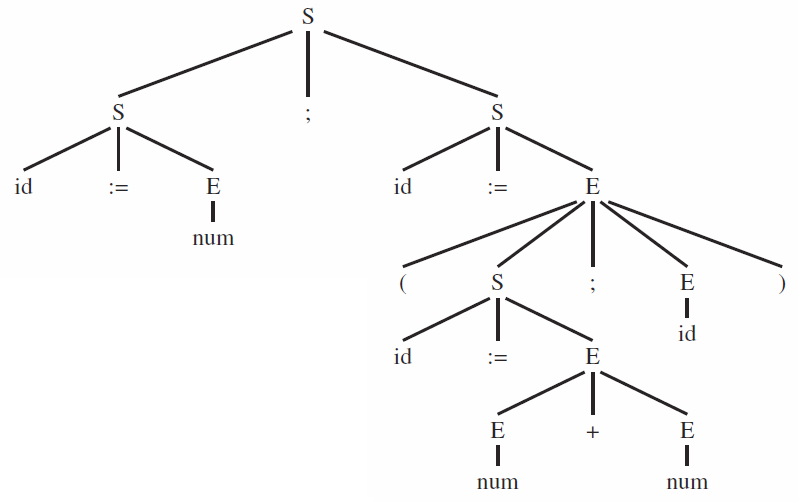
\includegraphics[width=\textwidth]{vb_tree_1}
	\caption{De bijhorende parse tree voor voorbeeldzin \ref{eqn:voorbeeldzin}.}
	\label{fig:vb_tree_1}
\end{figure}


\subsection{Ambigue grammatica}
\QA{Stel dat we Grammatica \ref{fig:vb_grammatica_1} hebben. Wat gebeurt er voor het statement \texttt{a := {\color{red}(}x + {\color{blue}(}y{\color{red})} + z{\color{blue})}}?}{Dit is een voorbeeld van een ambigue grammatica. Aan de hand van de grammatica is het onmogelijk om slechts één parse tree op te bouwen. Figuur \ref{fig:ambigious_grammar_tree} toont beide parse trees voor het statement. Bij de linkse boom worden de rode haakjes gebruikt terwijl be de rechtse boom de blauwe haakjes gebruikt worden.
}

\begin{figure}
	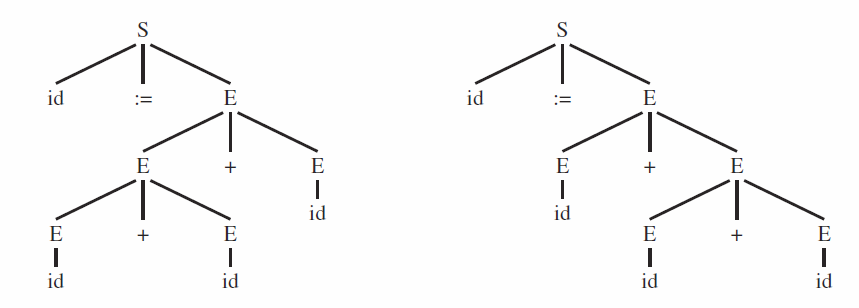
\includegraphics[width=\textwidth]{ambigious_grammar_tree}
	\caption{Voor Grammatica \ref{fig:vb_grammatica_1} kunnen er twee parse trees opgebouwd worden voor het statement \texttt{a := x + y + z}.} 
	\label{fig:ambigious_grammar_tree}
\end{figure}

Bij een plus-operatie is dit niet heel belangrijk aangezien het toch associatief is, maar bij niet-associatieve operaties is dit duidelijk niet goed.

\subsection{Grammatica disambiguëren}
Een grammatica hoeft niet perse de regels van de wiskunde te volgen. Daarom is het automatiseren ook moeilijk, omdat het afhangt van welke semantiek gewenst is. Er kan bijvoorbeeld gesteld worden dat:
\begin{itemize}
	\item * en / voorrang heeft op + en -,
	\item a + b + c = (a + b) + c, dus + is links associatief.
\end{itemize}
Om dit te realiseren worden er \textbf{termen} en \textbf{factoren} ingevoerd. Op die manier kan Grammatica \ref{grammar:3_5} omgevormd worden tot \ref{grammar:3_8}.

\begin{grammarfigure}
	\centering
	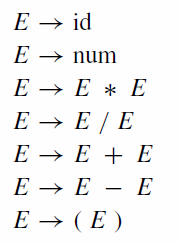
\includegraphics[width=0.25\textwidth]{grammar_3_5}
	\caption{Een ambigue grammatica. Hier wordt de regel dat * en / voorrang heeft op + en - niet gerespecteerd. }
	\label{grammar:3_5}
\end{grammarfigure}
\begin{grammarfigure}
	\centering
	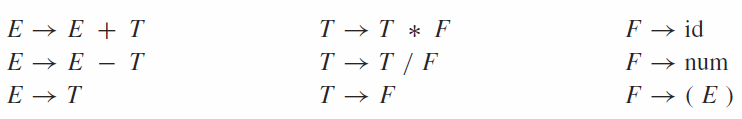
\includegraphics[width=\textwidth]{grammar_3_8}
	\caption{Grammatica \ref{grammar:3_5} kan hervormt worden, door termen $T$ en factoren $F$ in te voeren. Deze termen dwingen de volgorde van operaties en associativiteit vast.}
	\label{grammar:3_8}
\end{grammarfigure}


\section{Predictive Parsing}
Sommige grammatica's kunnen eenvoudig geparsed worden met een \textbf{recursive descent parser}. Voor elke niet-terminal is er een overeenkomstige functie. In elke functie is er een switch clause voor elke productieregel die door de niet-terminal kan gegenereerd worden. Niet-terminals worden recursief aangeroepen terwijl terminals verwerkt worden.

Code \ref{code:recursive_descent_parser} toont een voorbeld van zo een recursive descent parser toegepast op Grammatica \ref{grammar:3_11}.

\begin{grammarfigure}
	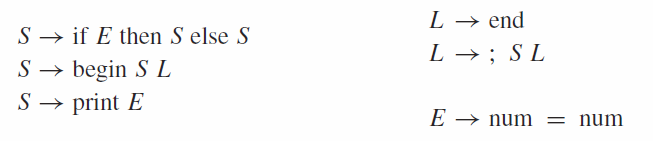
\includegraphics[width=\textwidth]{grammar_3_11}
	\caption{}
	\label{grammar:3_11}
\end{grammarfigure}

\begin{lstlisting}[caption={Een recursive descent parser gebaseerd op Grammatica \ref{grammar:3_11}},label={code:recursive_descent_parser},captionpos=b]
enum token {IF, THEN, ELSE, BEGIN, END, PRINT, SEMI, NUM, EQ};
extern enum token getToken(void);

enum token tok;
void advance() {tok = getToken();}
void eat(enum Token t) {if (tok==t) advance(); else error();}

void S(void) {switch(tok){
	case IF:    eat(IF); E(); eat(THEN); S(); eat(ELSE); S(); break;
	case BEGIN: eat(BEGIN); S(); L(); break;
	case PRINT: eat(PRINT); E(); break;
	default:    error();
}}
	
void L(void) {switch(tok){
	case END:  eat(END); break;
	case SEMI: eat(SEMI); S(); L(); break;
	default:   error();
}}

void E(void) {
	eat(NUM) ; eat(EQ) ; eat(NUM);
}
\end{lstlisting}

Een recursive descent parser werkt enkel als het eerste terminale symbool van een subexpressie genoeg informatie oplevert.

\subsection{First and follow sets}
Om de begrippen \textbf{first set} en \textbf{follow set} uit te leggen wordt Grammatica \ref{grammar:3_12} gebruikt.
\begin{grammarfigure}
	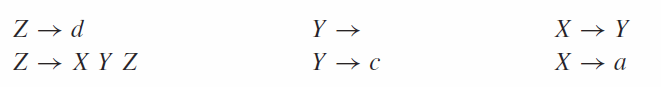
\includegraphics[width=\textwidth]{grammar_3_12}
	\caption{}
	\label{grammar:3_12}
\end{grammarfigure}
\begin{itemize}
	\item \textbf{nullable($X$)} $\rightarrow$ boolean: true als $X$ de lege string kan afleiden.
	
	We zien dat nullable($Y$) zeker waar is voor Grammatica \ref{grammar:3_12}. We kunnen echter vanuit $X$ ook naar de lege string gaan via $X \rightarrow Y \rightarrow \epsilon$, maar niet vanuit $Z$.
	
	\begin{table}[h]
		\centering
		\begin{tabular}{c | c c c}
	      & nullable & FIRST & FOLLOW \\
	      \hline
		X & yes & & \\
		Y & yes & & \\
		Z & no & & 
		\end{tabular}
	\end{table}
	
	\item \textbf{FIRST($\gamma$)}: verzameling terminals waarmee strings kunnen beginnen die van expressie $\gamma$ kunnen afgeleid worden.
	
	Uitgewerkt voor de drie startsymbolen:
	\begin{itemize}
		\item[$X:$] Vanuit $X$ zijn er twee mogelijkheden: $X \rightarrow a$ en $X \rightarrow Y$. We zien dat $a$ een terminal is dus die behoort al zeker tot de FIRST set. Vanuit $Y$ kan ook nog de lege string en $c$ bereikt worden. Hieruit volgt FIRST($X$) = $\{a\;c\}$.
		\item[$Y:$] Vanuit $Y$ kan enkel $c$ bereikt worden: FIRST($Y$) = $\{c\}$.
		\item[$Z:$] In eerste instantie kan $Z$ direct $d$ bereiken, dus die zit zeker in de FIRST set. Aangezien ook de productieregel $Z \rightarrow X\;Y\;Z$ bestaat en zowel $X$ als $Y$ nullable zijn, kan zowel de FIRST set van $X$ als van $Y$ overgenomen worden.
		
		FIRST($Z$) = $\{a\;c\;d\}$
	\end{itemize}

	\begin{table}[h]
	\centering
	\begin{tabular}{c | c c c}
			& nullable & FIRST & FOLLOW \\
			\hline
			X & yes & a c & \\
			Y & yes & c & \\
			Z & no & a c d & 
		\end{tabular}
	\end{table}
	
	\item \textbf{FOLLOW($X$)}: is de verzameling van terminals $t$ die meteen op $X$ kunnen volgen, dus waarvoor de afleiding $X_t$ bestaat. 
\end{itemize}

Algoritme \ref{algo:first_follow_nullable} is een fixpoint algoritme die de first, follow en nullable berekent.

\begin{lstlisting}[caption={Iteratieve berekening van FIRST, FOLLOW en nullable},label={algo:first_follow_nullable},captionpos=b,escapeinside={(*}{*)}]
(*\textbf{for}*) each terminal symbol Z
  FIRST[Z] (*$\leftarrow$*) {Z}
(*\textbf{repeat}*) 
  (*\textbf{for}*) each production (*$X \rightarrow Y_1Y_2...Y_k$*)
    (*\textbf{for}*) each (*$i$*) from 1 to (*$k$*), each (*$j$*) from (*$i + 1$*) to (*$k$*),
      (*\textbf{if}*) all the (*$Y_i$*) are nullable
        (*\textbf{then}*) nullable[X] (*$\leftarrow$*) true
      (*\textbf{if} $Y_1 \cdot\cdot\cdot Y_{i - 1}$*) are all nullable 
        (*\textbf{then}*) FIRST[X] (*$\leftarrow$*) FIRST[X] (*$\cup$*) FIRST[(*$Y_i$*)]
      (*\textbf{if} $Y_{i + 1} \cdot\cdot\cdot Y_{k}$*) are all nullable 
        (*\textbf{then}*) FOLLOW[(*$Y_i$*)] (*$\leftarrow$*) FOLLOW[(*$Y_i$*)] (*$\cup$*) FOLLOW[(*$X$*)]
      (*\textbf{if} $Y_{i + 1} \cdot\cdot\cdot Y_{j - 1}$*) are all nullable 
        (*\textbf{then}*) FOLLOW[(*$Y_i$*)] (*$\leftarrow$*) FOLLOW[(*$Y_i$*)] (*$\cup$*) FIRST[(*$Y_i$*)]
(*\textbf{until}*) FIRST, FOLLOW and nullable did not change in this iteration
\end{lstlisting}



\subsection{Opstellen Predictive Parsing Tabel}
Uitbreiden definitie van first naar strings:
\begin{itemize}
	\item \texttt{FIRST($W\gamma$)} = \texttt{FIRST($W$)} als niet nullable($W$)
	\item \texttt{FIRST($W\gamma$)} = \texttt{FIRST($W$)} $\cup$ \texttt{FIRST($\gamma$)} 
\end{itemize}


Er zijn drie gevallen waarbij er twee keuzes zijn. Moeten we $X \rightarrow a$ of $X \rightarrow Y$ nemen? De string $d$ levert minstens twee parse tree op. De grammatica was zelfs ambigu. Dit kan nooit geparsed worden.

\subsection{LL(1) Parsers}
\begin{itemize}
	\item Elk vak in de tabel bevat slechts 1 productieregel.
	\item Left-to-right parse: begin vooraan in broncode en verwerk van links naar rechts. 
	\item Leftmost-derivation: 
	\item 1-symbol lookahead: Er wordt slechts één symbool vooraf bekeken.
	\item LL($k$):
	\begin{itemize}
		\item $k$ symbolen vooraf bekijken. De first sets bevatten sequenties van $k$ terminals.
	\end{itemize}
	\alert Mogelijke problemen:
	\begin{itemize}
		\item Linkse recursie.
		\begin{itemize}
			\item Probleem: zekerheid van meerdere productieregels in een vak want $\texttt{FIRST(T)} \in \texttt{FIRST(E - T)}$. 
			\item Oorzaak: $E$ verschijnt links in de rechterkant van een $E$-productie.
			\item Oplossing: 
		\end{itemize} 
		\item Linkse factorisatie.
		\begin{itemize}
			\item Probleem: De parser kan geen onderscheid maken tussen twee gelijkaardige strings.
			\item Oplossing: grammatica herschrijven.
		\end{itemize}
	\end{itemize}
	\item Error recovery is mogelijk.
	\alert Beslissing nemen na $k$ symbolen blijft een zwakte.
	
\end{itemize}

\subsection{Error Recovery}
Probleem: pseudocode voor error. We willen geen compiler die geen nuttige foutboodschappen kan geven. Compiler mag ook niet stoppen bij eerste fout, omdat meerdere fouten nog verder kunnen voorkomen.
\begin{itemize}
	\item Gewoon een print statement = vrij slechte methode aangezien er geen tokens opgegeten worden. De parser doet voort alsof hij F en Tprime al geparsed heeft. De parser komt in foute toestand.
	\item Print statement combineren met de skipto functie, die tokens zal opeten totdat er een token tegenkomt die in de follow set zit. Alle karakters die niet in de follow zitten, zal nog deel uitmaken van de subexpressie. 
\end{itemize}

\section{LR(1) parser}
\begin{itemize}
	\item Left-to-right parse
	\item Rightmost-deviation
\end{itemize}
	\chapter{Abstracte syntax}
\label{ch:abstract_syntax}
Abstract syntax tree stelt eerder semantiek voor, parse trees de constructieregels. De abstract syntax tree wordt opgebouwd tijdens het parsen.
\section{Semantische acties}


Een parser voert syntactische acties uit zoals shift en reduce. Een semantische actie heeft betrekking tot de betekenis van de expressies. Het bereken van semantische waarden kan bv zijn:
\begin{itemize}
	\item het type van het linkerlid van de expressie $a = 5 + 3$ bepalen.
\end{itemize}


\subsection{Voorbeeld}
\begin{enumerate}
	\item Rekenmachine: Specifieren tokens van verschillende types (bv token type id komt overeen met strings). 
	
	Eerst $a = 5$, dan $c = a + b$, dan moet $a$ eerst opgezocht worden (lookup).
	
	Elke terminal heeft een type semantische waarde, en is dan ook returntype van de functie voor die terminal.
	
	
	\item Betere rekenmachine: niet manueel implementeren maar met tool (bv Yacc)
	
	\$\$ is de semantische waarde van het linkerlid
	
	\$1 is de semantische waarde van de eerste expressie in de tokenlijst.
	
	Figuur 4.3
	
	Semantische waarde van $exp$ is semantische waarde van $INT$
	
	Opt einde: reductie van \texttt{exp TIMES exp}
	\item Interpreter
\end{enumerate}
In feite kan compilatie uitgevoerd worden met semantische acties, maar wordt in de praktijk afgeraden:
\begin{itemize}
	\item Analyse kan enkel uitgevoerd worden in de volgorde dat de inputstream geparsed wordt. 
	\item Code genereren op basis van parse tree, maar zo een tree is niet geschikt. Er zit te veel nutteloze informatie in zoals := operator, en dient eerder om de syntax uit te drukken en niet semantiek.
\end{itemize}

\section{Abstract Parse Tree Construction}

Grammatica 4.5 is ambigue. Binaire operator specificeert geen associativiteit. Dit is geen probleem, aangezien de parser dit al beslist heeft. Dus de grammatica die de parser gebruikt mag niet ambigue zijn, wel die van de abstract syntax tree, aangezien die dient om de semantiek te definiëren.
\subsection{Posities}
Als je tree opbouwt, wordt deze geanalyseerd om bv types te checken. Bij foutboodschappen moet de compiler weten waar in de inputstroom deze fout gegenereerd wordt. Er kan een \textbf{positiestack} bijgehouden worden die de positie van elke token bevat.
	\chapter{Semantische analyse}
\label{ch:semantische_analyse}

\begin{lstlisting}
int b = 0;
extern int a;
void foobar(float b){
  if(b == 0.0){
    char * b = malloc(1);
    *b = 0;
  }
}
\end{lstlisting}

Er wordt een nullbyte weggeschreven naar $b$. Is dit een string, float, 32 bit integer, 64 bit integer? Het algemene probleem is dat er verschillende scopes zijn, en binnen elke scope kan dezelfde variabele identifier gebruikt worden. Via \textbf{symbooltabellen} wordt dit efficiënt opgelost.
\section{Symbooltabellen}
Een symbooltabel bestaat uit een \textbf{environment} $\sigma_i$ en een verzameling \textbf{bindings}.
$$\sigma_1 = \{g \rightarrow string, a \rightarrow int}$$

Elke environment $\sigma_i$ bestaat uit de samenstellingen van zijn specifieke bindings en eventueel de bindings van andere $\sigma_{j}$ voor $j \neq i$. De specifieke bindings van $\sigma_i$ hebben voorrang op de bindings van $\sigma_{j}$.

\underline{Twee implementaties:}
\begin{itemize}
	\item \textbf{Imperatieve implementatie:} Er wordt een hashtabel bijgehouden waarin kan toegevoegd en opgezocht worden. Er is geen remove operatie maar wel een pop operatie aangezien elke bucket kan gezien worden als een stapel omdat geneste expressies nooit overlappen. Elke bucket van de hashtabel is een scope.
\item \textbf{Functionele implementatie:} Kopieërt niet de hele hashtabel, maar enkel de pointers naar de relevante buckets. Kan met hashtabel, maar (zelfbalanserende) binaire zoekbomen zijn efficiënter.
\end{itemize}
\subsection{Efficiëntere symbooltabellen}
Tabel aanmaken met pointers naar identifier tijdens het parsen., in plaats van "a" op AST figuur 1.4 wordt de pointer bijgehouden in de knoop.   
(slide 15)


\section{Type Checking}
Kijken of de gebruikte veranderlijken:
\begin{itemize}
	\item gedeclareerd zijn
	\item ze van het juiste type zijn
	\item of de types van expressies correct zijn
\end{itemize}
Door de abstract syntax tree in postorder te overlopen kan dit geïmplementeerd worden. Er zullen altijd eerst declaraties bezocht worden. Er zijn verschillende visitors 
\subsection{Expressies}

\subsection{Variabelen}

\subsection{Declaraties}


	\chapter{Activation Records}
Er is een overstap nodig naar een neutrale voorstelling die onafhankelijk is van de oorspronkelijke taal. Er is wel een probleem: zelfs de omzetting van de abstract syntax tree naar deze neutrale voorstelling is afhankelijk van de architectuur waarvoor gecompileerd wordt. Bijvoorbeeld het statement \texttt{*p++} in C is anders voor 32-bit of 64-bit systemen. Het doel is om de taalspecifieke Abstract Syntax Tree om te vormen naar een taalonafhankelijke Intermediate Representation Tree.

Bij de meeste talen worden er lokale variabelen gecreëerd bij het aanroepen van een functie. Meerdere instanties van een functie kunnen bestaan en hebben elk hun eigen instanties van lokale variabelen.
\begin{lstlisting}
function f(x: int) : int =
  let var y := x + x
   in if y < 10
          then f(y)
          else y - 1
end
\end{lstlisting}
Een instantie van $x$ wordt aangemaakt elke keer dat $f$ opgeroepen wordt. Door de recursiviteit kunnen er meerdere instanties van $x$ bestaan. Een functieoproep heeft een last-in-first-out (LIFO) gedrag. Alle lokale variabelen binnen een functie worden vernietigd op het moment dat deze functie verlaten wordt. De gebruikte datastructuur is dus een \textbf{stack}.

Een hogere orde functie is een functie waarin:
\begin{itemize}
	\item een andere functie aanwezig is.
	\item een functie heeft als returnwaarde.
	\item Voorbeeld:
	\begin{lstlisting}
fun f(x) =
 let fun g(y) = x + y
  in g
 end
 
val b = f(3)
val j = f(4)
	
val z = h(5)
val w = j(7)
	\end{lstlisting}
	\good 	Zulke functies worden niet besproken in deze cursus.
\end{itemize}




\section{Stack Frames}
\begin{itemize}
	\item Een normale stack kent twee operaties: \textbf{push} en \textbf{pop}.
	\item \textbf{Problemen:}
	\begin{itemize}
		\item Lokale variabelen worden in grote hoeveelheden op de stack geplaatst. 
		\item Lokale variabelen zijn niet altijd geïnitialiseerd.
		\item Ook al zijn de variabele gepushed, is er nog steeds random access nodig.
	\end{itemize}  
	\item \textbf{Oplossing:} De stack als een array beschouwen met een speciaal register - de stack pointer. Elke lokatie na de stack pointer is rommel, alles ervoor is gealloceerd.
	\item Het gebied op de stack voor een functie $f$ die zijn lokale variabelen, parameters, returnadres en andere temporaries bevat wordt een \textbf{activation record} of \textbf{stack frame} genoemd.
\end{itemize}



Wat is het verschill tussen een caller-safed register en een callee-saved register?
\begin{lstlisting}
	ADD		R1, R2, R3 // R1 = R2 + R3
	CALL	F
	MUL		R4, R1, R7 // R4 = R1 * R7
	\end{lstlisting}
	Gaat F de waarde R1 overschrijven of niet? Als dit onbepaald is, is het geen geldige code. Een callee-saved register is de restrictie dat F deze waarde niet kan aanpassen. Een caller-safed register legt de restrictie op aan de caller van F. De assembly moet dan uitgebreidt worden:
	\begin{lstlisting}
	ADD		R1, R2, R3
	ST		R1, SP[...] // store R1 
	CALL	F
	LD      R1, SP[...] // load R1
	MUL		R4, R1, R7
	\end{lstlisting}
	Een deel van de registers worden caller-safed gemaakt, de rest is dan callee-safed. Dit wordt manueel vastgelegd. De compiler kan dan oproepen optimaliseren.






\begin{figure}
	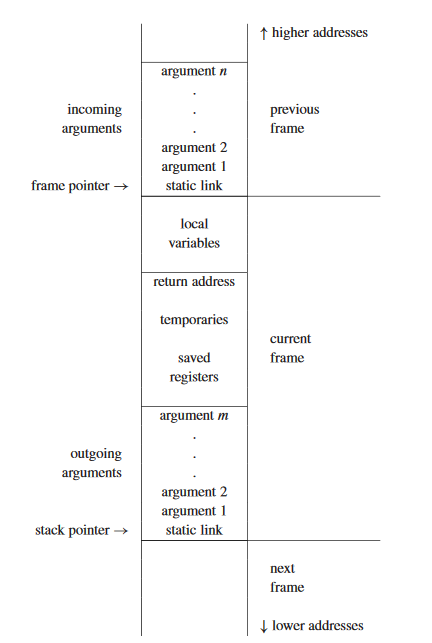
\includegraphics[width=\textwidth]{frame_layout}
	\caption{Een stack frame.}
	\label{fig:stack_frame}
\end{figure}



\subsection{Static Link}

De stack kan ook argumenten bevatten die meegegeven worden aan de functie. Een static link is vooral belangrijk bij geneste en recursieve functies. In program 6.3 (slide 6) moet de variabele \texttt{output} in elke frame beschikbaar zijn. De static link bevat een pointer naar de buitenste functie, zodat deze variabele in elke geneste functie beschikbaar is.



\subsection{Escapes}
Een variable \textit{escapet} uit een stack frame als:
\begin{itemize}
	\item hij passed-by-reference wordt.
	\item of zijn adres genomen wordt.
	\item of hij geaccessed wordt vanuit een geneste functie.
\end{itemize}

Een veranderlijke is \textit{memory-resident} (in het geheugen steken) als
\begin{itemize}
	\item hij escapet
	\item of niet in een register past
	\item of een array is
	\item of er geen vrij register is
\end{itemize}

Welke parameters moeten op de stack frame zitten en welke niet? Stel volgende functie:
\begin{lstlisting}
int f(int x, int y){
  f(x);
  g(&x);
  return x + y;
}
\end{lstlisting}
Als de functieoproepen $f$ en $g$ er niet zijn, dan moeten $x$ en $y$ niet op de stack. Bij de functie $f$ hangt het af of dat $f$ de parameter aanpast. Bij de functie $g$ moet $x$ zeker in het geheugen zitten en zal dus niet op de stack komen.
\begin{lstlisting}
int f(int x, int y){
  p = &x;
}
\end{lstlisting}


\section{Frames in de Tiger compiler}
\subsection{Frame Interface}
Er is een abstracte representatie nodig van een frame want deze hangt af van de architectuur. Deze komt in \texttt{frame.h}.

\begin{itemize}
	\item \texttt{F\_frame}: datastructuur die een frame voorstelt. 
	\item \texttt{F\_access}: datastructuur die specifieert hoe lokale variabelen moeten geaccesseerd worden (register of geheugen).
	\item \texttt{F\_accessList}: Lijst van \texttt{F\_access} structuren.
	\item \texttt{newFrame(Temp\_label name, U\_boolList formals)}: formals bevat booleans die voor elke parameter aangeeft of hij deze escapet moet worden of niet.
	\item \texttt{allocLocal(F\_frame f, bool escape)}: maakt plaats voor nieuwe veranderlijke in frame $f$, en eventueel wordt hij in het geheugen geplaatst in plaats van de stack.
\end{itemize}

Voorbeeld:
\begin{lstlisting}
F_Frame frame = F_frame(g, U_BoolList(TRUE,
                              U_BoolList(FALSE,
                                 U_BoolList(FALSE,NULL))))
\end{lstlisting}
 
\subsection{Creatie en initialisatie van frames}
\begin{figure}
	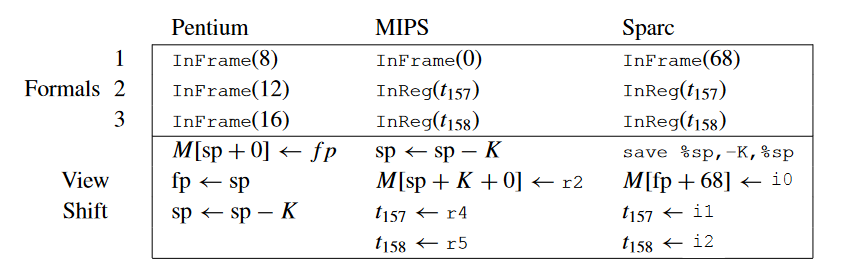
\includegraphics[width=\textwidth]{create_frames}
	\caption{Formele parameters voor $g(x_1, x_2, x_3)$ waarbij $x_1$ escapes.}
	\label{fig:create_frames}
\end{figure}

Bij Pentium moet alles op de stack. In MIPS wordt standaard de eerste 3 argumenten in registers gestoken, maar $x_1$ escapet dus wordt hij in het geheugen bewaard.
 
 \subsection{Escapes berekenen}
 Een variable \textit{escapet} uit een stack frame als:
 \begin{itemize}
 	\item hij passed-by-reference wordt.
 	\item of zijn adres genomen wordt.
 	\item of hij geaccessed wordt vanuit een geneste functie.
 \end{itemize}
 Pass-by-reference of het nemen van een referentie is direct zichtbaar in de Abstract Syntax Tree. Om na te gaan of hij geaccessed wordt vanuit een geneste functie wordt de Abstract Syntax Tree recursief overlopen met een symbooltabel (omgeving), maar hier zijn alle veranderlijken gebonden aan booleans: escapes of niet. Deze stap wordt voor semantische analyse en na parsing gedaan. Dus tussen deze twee stappen worden de escapes berekent. Het kan ook efficiënter, maar zien we niet in deze cursus.
 
\subsection{Temporaries en Labels}
\begin{itemize}
	\item Een \textbf{temporary} is een waarde die tijdelijk in een nog te bepalen register wordt bewaard.
	\item Een \textbf{label} is een nog onbekend adres waarde code of statisch gealloceerde data zal terecht komen. Bijvoorbeeld \texttt{string = \textquotedblright een string\textquotedblright} wordt statisch gealloceerd.
	\item Er is ook een aparte interface \texttt{temp.h}.
\end{itemize} 

	
\chapter{Intermediate Representations}
\begin{figure}[ht]
	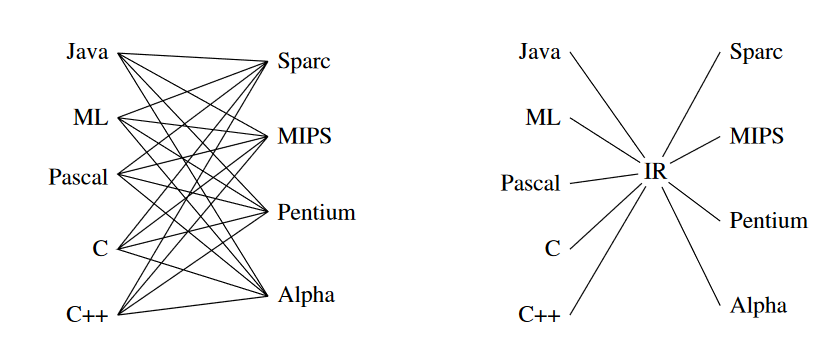
\includegraphics[width=\textwidth]{intermediate_representations}
	\caption{Compilers voor vijf talen en vier architecturen: 
		(links) geen IR, (rechts) met IR.}
	\label{fig:intermediate_representations}
\end{figure}
Een goede IR moet:
\begin{itemize}
	\item makkelijk te produceren zijn door de compiler frontend
	\item makkelijk zijn om er echte assembler van te genereren
	\item duidelijke, eenvoudige betekenis hebben
\end{itemize}

Een IR-tree is een eenvoudige abstractie van machine-instructies. Het lijkt heel goed op een Abstract Syntax Tree maar is taal-onafhankelijk en werkt met temporaries in plaats van variabelen.

Typen van expressies (\texttt{T\_exp}):
\begin{itemize}
	\item \texttt{CONST(i)}: integer constante $i$
	\item \texttt{NAME(n)}: assembly label $n$
	\item \texttt{TEMP(t)}: virtueel register $t$
	\item \texttt{BINOP(o, $e_1$, $e_2$)}: $e_1 o e_2$ met $o = +, -, *, /, ...$. Hier wordt $e_1$ altijd eerst geëvalueerd.
	\item \texttt{MEM(e)}: De inhoud van $w$ bytes op $e$ schrijven of lezen.
	\item \texttt{CALL(f, $l_1, ..., l_n$)}: roep $f$ op met argumenten $l_i$. De volgorde van de argumenten is van belang.
	\item \texttt{ESEQ(s, e)}: evalueer $s$ voor neveneffecten, dan $e$ als resultaat.
\end{itemize}

Typen van statements:
\begin{itemize}
	\item \texttt{MOVE(TEMP t, e)}: evalueer $e$ en wijs toe aan temp $t$.
	\item \texttt{MOVE(MEM($e_1$), $e_2$)}: evalueer $e_1$ tot adres $a$, evalueer $e_2$ en schijf het in de $w$ bytes vanaf $a$.
	\item \texttt{EXP(e)}: evalueer $e$ en negeer het resultaat.
	\item \texttt{JUMP(e, labs)}: evalueer $e$ tot een adres en spring er naar. 
	\item \texttt{CJUMP(e ...)}:
	\item \texttt{SEQ($s_1$, $s_2$)}: sequentie van statements 
\end{itemize}

Er is geen 1-op-1 mapping van \texttt{A\_EXP} naar \texttt{T\_EXP}.

\QA{Waarom staan er NULL pointers?}{We weten nog niet naar waar we moeten springen. Er moeten labels inkomen, maar we kennen ze nog niet. Voorlopig dienen die dus als placeholders.}

patchlist bevat de labels (in gelinkte lijst vorm) in geval van true en geval van false. De constructor bevat het hele pad in de IR tree naar het lege veld vanaf de root van het statement ($s_1$ in voorbeeld). Als de waarde 0 of 1 in \texttt{flag} moet komen kan de expressie geconverteerd worden naar een andere expressies. Program 7.3: steek 1 in temporary, als we false uitkomen wordt 0 in temporary gestoken. De doPatch functie kent een label toe aan een bepaald veld in de boom.

\subsection{Omzetting enkelvoudige veranderlijken}

$+$ symbool is dereference operator


l-values:
\begin{itemize}
	\item kan links in een toewijzing voorkomen
	\item verwijst naar een locatie
\end{itemize}

r-values:
\begin{itemize}
	\item kan enkel rechts in een toewijzing voorkomen
	\item verwijst impliciet naar een waarde
\end{itemize}

scalar:
\begin{itemize}
	\item Waarde die slechts één geheugenwoord bevat.
\end{itemize}




	\part{Oefeningensessies}
	\chapter{Oefeningensessie 1}

\section{Oefening 3.6 p85}
Gegeven de volgende grammatica:
\begin{equation*}
	\begin{split}
	& S \mapsto uBDz \\
	& B \mapsto Bv \\
	& B \mapsto w \\
	& D \mapsto EF \\
	& E \mapsto y \\
	& E \mapsto \\
	& F \mapsto x \\
	& F \mapsto 
	\end{split}
\end{equation*}
\begin{enumerate}
	\item \textbf{Bereken nullable, FIRST en FOLLOW.}
	\begin{table}[h]
		\centering
		\begin{tabular}{| l | c | c | c |}
			\hline
			& nullable & FIRST & FOLLOW \\
			\hline
			S & nee & \{ u \}    & /	 			\\
			B & nee & \{ w \}    & \{ x, y, v, z \}	\\
			D & ja  & \{ x, y \} & \{ z \}			\\
			E & ja  & \{ y \}    & \{ x, z \}		\\
			F & ja  & \{ x \}    & \{ z \}			\\
			\hline
		\end{tabular}
	\end{table}

	\item \textbf{Construeer de $LL(1)$ parsingtabel.}
	\begin{table}[h]
		\centering
		\begin{tabular}{| l | l | l | l | l | l | l |}
			\hline
			   & u 					& z & v & w & y & x \\
			 S & $S \mapsto uBDz$  	&   &   &   &   &   \\
			 B &   					&   &   & $B \mapsto w, \; B \mapsto Bv$  &   &   \\
			 D &  					& $D \mapsto EF$  &   &   & $D \mapsto EF$  & $D \mapsto EF$   \\
			 E &   					& $E \mapsto $  &   &   & $E \mapsto y$  &  $E \mapsto $ \\
			 F &   					& $F \mapsto $  &   &   &   &  $F \mapsto x$ \\
			\hline
		\end{tabular}
	\end{table}

	\item \textbf{Toon aan dat dit geen $LL(1)$ parser is.}
	
	Als we B aan het parsen zijn, en het eerstvolgende token is een $w$ dan weten we niet welke productieregel toegepast moet worden.
	
	\item \textbf{Wijzig de grammatica \emph{zo weinig mogelijk} om een $LL(1)$ grammatica te hebben dat dezelfde taal aanvaardt.}
	
	Door de linkse recursiviteit van de productieregel $B \mapsto Bv$, kunnen volgende veranderingen ingevoerd worden:
	\begin{equation*}
		\begin{split}
		& B \mapsto wB' \\
		& B' \mapsto vB' \\
		& B' \mapsto 
		\end{split}
	\end{equation*}
\end{enumerate}

\section{Voorbeeldexamenvraag}
Gegeven de reguliere expressie $S = ab+c$.
\begin{enumerate}
	\item \textbf{Schrijf een (ambigue) grammatica voor $S$ met tokens $a$, $b$ en $c$.}
	
	\begin{equation*}
		\begin{split}
	& S' \mapsto S \& \\
	& S \mapsto aBc \\
	& B \mapsto bB \\
	& B \mapsto b 
		\end{split}
	\end{equation*}
	
	\item \textbf{Geef de $LR(0)$ statentabel en $LR(0)$ parsingtabel.}
	
	Altijd de closure nemen van productieregel van niet-terminal waar het puntje voor staat. dus alle productieregels opnemen in toestand van die niet-terminal. Uiteindelijk moet elk puntje op het einde staan.
	
	\begin{figure}[ht]
		\centering
		\begin{tikzpicture}[state/.style={rectangle, draw, inner sep = 2mm}]
		\node (1) [state] {$\begin{aligned}S' \mapsto& .S\$ \\ S \mapsto& .aBc\end{aligned}$};
		\node (2) [state, right = 1.5cm of 1] {$S \mapsto S.\$$};
		\node (3) [state, below = 1cm of 1] {$\begin{aligned}
			S \mapsto& a.Bc \\
			B \mapsto& .bB \\
			B \mapsto& .b
			\end{aligned}$};
		\node (4) [state, right = 1.5cm of 3] {$\begin{aligned}
			S \mapsto& aB.c
			\end{aligned}$};
		\node (7) [state, right = 1.5cm of 4] {$\begin{aligned}
			S \mapsto& aBc.
			\end{aligned}$};
		\node (5) [state, below = 1cm of 3] {$\begin{aligned}
			B \mapsto& b.B \\
			B \mapsto& b. \\
			B \mapsto& .bB \\
			B \mapsto& .b
			\end{aligned}$};
		\node (6) [state, right = 1.5cm of 5] {$\begin{aligned}
			B \mapsto& bB. 
			\end{aligned}$};
		
		\draw [->] (1) -- node[yshift=0.25cm] {S} (2);
		\draw [->] (1) -- node[xshift=0.25cm] {a} (3);
		\draw [->] (3) -- node[yshift=0.25cm] {B} (4);
		\draw [->] (3) -- node[xshift=0.25cm] {b} (5);
		\draw [->] (4) -- node[yshift=0.25cm] {c} (7);
		\draw [->] (5) -- node[yshift=0.25cm] {B} (6);
		\path [->] (5) edge[loop left] node[yshift=0.25cm] {c} ();
		
		\node (label1) [anchor=north east, inner sep = 1pt] at (1.north east) {\textbf{1.}};
		\node (label1) [anchor=north east, inner sep = 1pt] at (2.north east) {\textbf{2.}};
		\node (label1) [anchor=north east, inner sep = 1pt] at (3.north east) {\textbf{3.}};
		\node (label1) [anchor=north east, inner sep = 1pt] at (4.north east) {\textbf{4.}};
		\node (label1) [anchor=north east, inner sep = 1pt] at (5.north east) {\textbf{5.}};
		\node (label1) [anchor=north east, inner sep = 1pt] at (6.north east) {\textbf{6.}};
		\node (label1) [anchor=north east, inner sep = 1pt] at (7.north east) {\textbf{7.}};
		\end{tikzpicture}
	\end{figure}

	
	\begin{table}[h]
		\centering
		\begin{tabular}{| l  | l | l | l | l | l | l |}
			\hline
			  & a & b & c & \$ & S & B \\
			  \hline
			1 & s3  &   &   &    & g2\footnote{Als er een reductie uitgevoerd is in toestand 1 voor $S$, dan moeten we naar toestand 2 gaan}   &   \\
			2 & & & & & & \\
			3 & & s5\footnote{Als we $b$ shiften uit toestand 3 zitten we in toestand 5} & & & & g4 \\
			4 & & & s7 & & & \\
			5 & r3\footnote{Reductie kan uitgevoerd worden met regel 3 ($B \mapsto b$)} & s5,r3 & r3 & r3 & & g6 \\
			6 & r2 & r2 & r2 & r2 & & \\
			7 r1 & r1 & r1 & r1 & & & \\
			\hline
		\end{tabular}
	\end{table}

	\item \textbf{Zijn er conflicten? Waarom wel of niet?}
	
	Er is een shift-reduce conflict voor toestand 5 en token $b$. Dit komt omdat de gekozen grammatica ambigue is.

	\item \textbf{Construeer een niet-ambigue LL parsingtabel die deze expressie herkent. Indien nodig, maak de grammatica niet-ambigue.}
		
		Grammatica herschrijven:
	\begin{equation*}
	\begin{split}
	& S \mapsto aBc \\
	& B \mapsto bB' \\
	& B' \mapsto  \\
	& B' \mapsto B 
	\end{split}
	\end{equation*}
	
	nullable, FIRST en FOLLOW bepalen:
	\begin{table}[ht]
		\centering
		\begin{tabular}{| l | l | l | l |}
			\hline
			& nullable & FIRST & FOLLOW \\
			\hline
			S & nee  & \{ a \}    & /	 			\\
			B & nee  & \{ b \}    & \{ c \}	\\
			B' & ja  & \{ b \}    & \{ c \}			\\
			\hline
		\end{tabular}
	\end{table}

	$LL(1)$ parsing table opstellen:
	
	\begin{table}[h]
		\centering
		\begin{tabular}{| l | l | l | l |}
			\hline
			  & a 					& b & c \\
			  \hline
			S & $S \mapsto aBc$	    &   &   \\
			B &   					& $B \mapsto bB'$  &   \\
			B' &  & $B' \mapsto B$ & $B' \mapsto$ \\
			\hline
		\end{tabular}
	\end{table}
	
\end{enumerate}

\section{Oefening 3.13 p86}
Toon aan dat de volgende grammatica $LALR(1)$ is maar niet $SLR$:
\begin{equation*}
\begin{split}
0 :& S \mapsto X\& \\
1 :& X \mapsto Ma \\
2 :& X \mapsto bMc \\
3 :& X \mapsto dc \\
4 :& X \mapsto bda \\
5 :& M \mapsto d
\end{split}
\end{equation*}


\end{document}